\chapter{Travail réalisé}
Avant de commencer, je vous présente mon travail sur le sujet du stage.\\[0.2cm]
Dans un premier temps, il faudra installer le système Raspbian. Une fois l’installation faire, il faudra configurer le système. Avant de commencer l’application, il me faudra faite quelques tests afin de vérifier le bon fonctionnement. Une fois cela terminé, il me faut vérifier que la caméra fonctionne correctement.

    \section{Mon travail}
    % Présentation du travail a effectuer sur le projet.
    \begin{flushleft}
        % A faire |!|
        Ma mission est de réaliser l'installation et de configurer un dispositif de capture vidéo réalisé par un \textit{Raspberry Pi} ainsi que de développer une application conviviale pour la gestion des vidéos.\\[0.2cm]
    
        % A revoir |!|
        Dans un premier temps, il faudra installer le système Raspbian.
        Une fois l'installation faite, il faudra configurer le système.
        Avant de commencer l'application, il me faudra faire quelques tests afin de vérifier le bon fonctionnement.
        Une fois cela terminé, il me faut vérifier que la caméra fonctionne correctement.    
    \end{flushleft}

    \section{Réception du matériel}
        \subsection{Raspberry Pi}
        Le \textit{Raspberry Pi} est un ordinateur portable de petite taille, doté d'un processeur ARM et d'un système d'exploitation Linux.

        % Intérêt :
        % - cout, manipulation
        % Inconvénients :
        % - la qualité ?
        % - configuration pas toiujours simple - fragile

        % Raspberry Pi 4 Model B :

        \vspace{0.2cm}

        \begin{flushleft}
            \begin{itemize}
                \item \textbf{Intérêt :}
                Le principal intêret de ce type de matériel est son coût qui est très faible. Comme le montre le tableau ci-dessous.
            \end{itemize}                       

            \begin{center}
                \begin{tabular}{ |p{3cm}|p{3cm}|p{3cm}|p{3cm}|  }
                    \hline
                    Nom & Processeur & RAM & Prix\\
                    \hline
                    Raspberry Pi 2w & 1.5 GHz Quad-Core A72 & 512Mb & 15€\\
                    \hline
                    Raspberry Pi 3 & 1.4 GHz Quad-Core A53 & 1Gb & 35€\\
                    \hline
                    Raspberry Pi 4 & 1.8 GHz Quad-Core A72 & 2Gb & 45€\\
                    \hline
                \end{tabular}            
            \end{center}

            Le Raspberry Pi est également simple à manipuler. Néamoins il possède certains Inconvénients.

            \begin{center}
                \begin{itemize}
                    \item \textbf{Inconvénients :}
                    En vu de sa petite taille, il est très fragile mais égalemnt très peu performant.
                    Sa configuration n'est pas toujours simple à réaliser.
                    Nous pouvons toujours augmenter les performances du Raspberry Pi via à de l'\underline{Overclocking} mais il faudrait un système de refroidissement pour le Raspberry Pi.
                \end{itemize}
            \end{center}



        \end{flushleft}     
            
        \begin{figure}[ht]
            \centering
            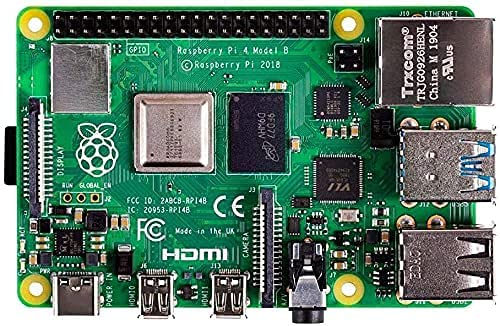
\includegraphics[scale=0.2]{rasp.jpg}
            \caption{Raspberry Pi 4}
        \end{figure}
        
 
        \subsection{Ecran LCD (Raspberry Pi)}
        Avec le \textit{Raspberry Pi} un écran LCD de 7 pouces permettant d'interagir avec l'ordinateur grâce à son écran tactile. 

        \begin{flushleft}
            L'Intérêt majeur de ce type de périphérique c'est sa finesse.
            En effet, dans un laboratoire il est pas toujours facil d'avoir un grand écran.
            De ce fait avoir un écran de petite taille qu'on peut tenir dans nos main tout en ayant la possibilité d'utiliser l'écran tactile pour interagir avec l'ordinateur nous permettant de nous dispenser de clavier et de souris.
        \end{flushleft}

        \begin{figure}[ht]
            \centering
            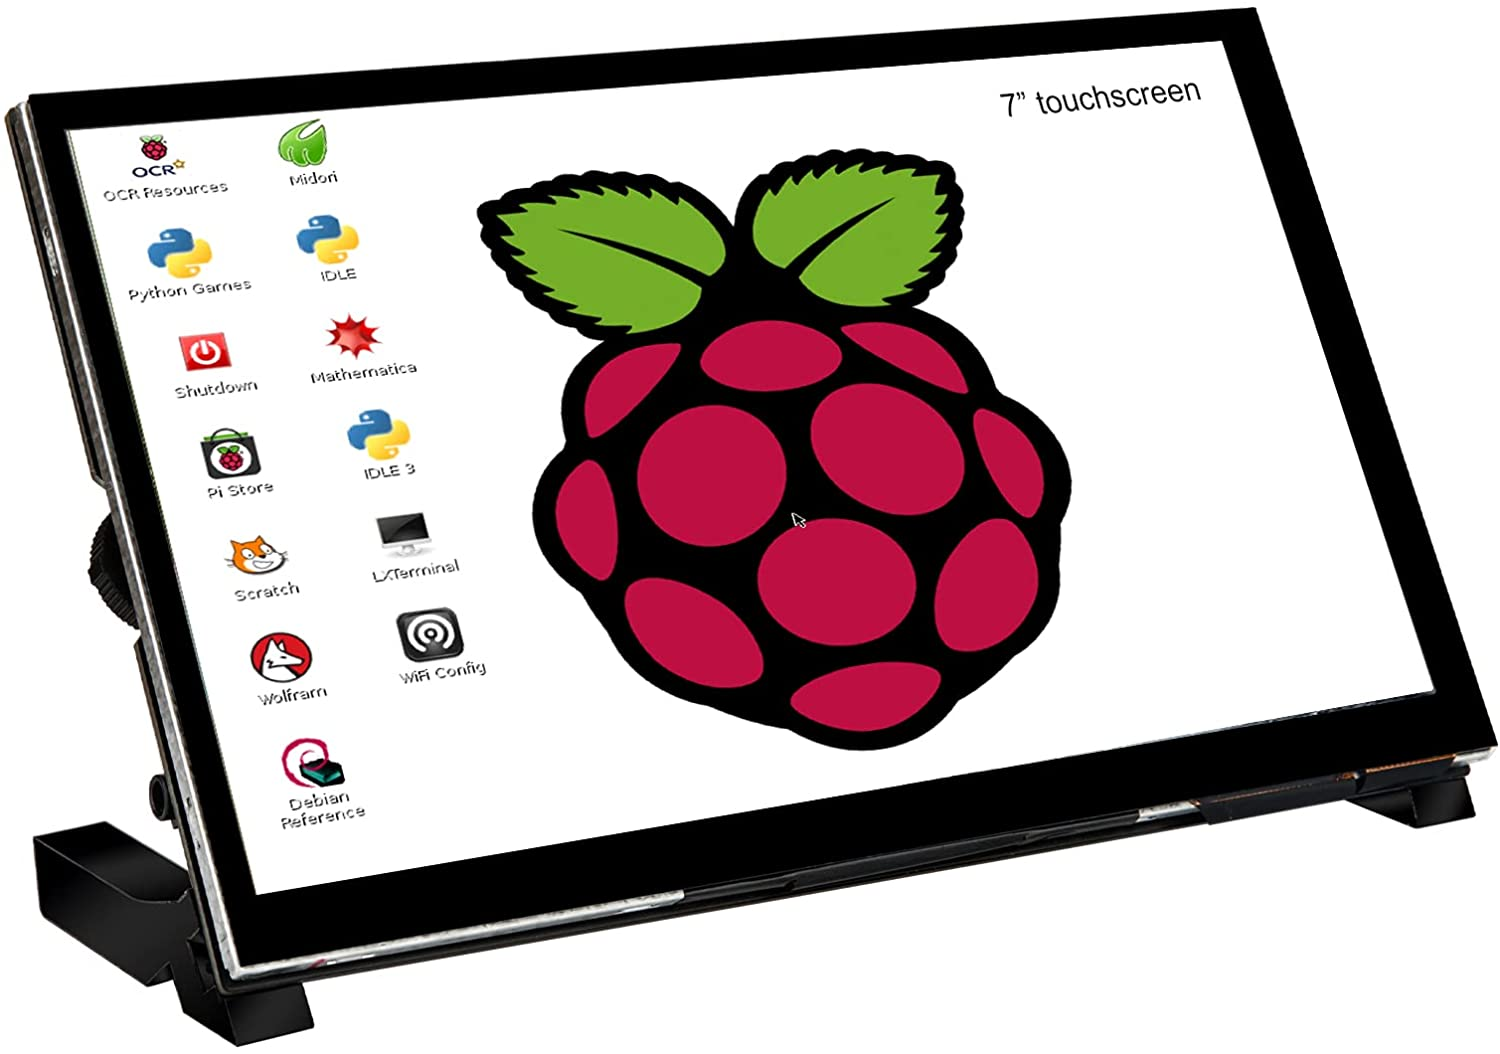
\includegraphics[scale=0.05]{ecran7p.jpg} 
            \caption{Ecran LCD de 7 pouces}
        \end{figure}

        \vspace{1cm}

        \subsection{Module de capture vidéo (Raspberry Pi) V2}
        Le module de capture vidéo (Raspberry Pi) V2 est un module de captation vidéo qui permet de capturer des images et des vidéos.

        % intérêt :
        % - cout, manipulation
        % Inconvénients :
        % - la qualité ?
        % - configuration pas toiujours simple - fragile

        \begin{flushleft}
            \begin{itemize}
                \item \textbf{Intérêt :}
                Le principal Intérêt de ce module est son coût qui est très faible. De plus tout comme le Raspberry Pi, il est très facile a manipuler. 
                \item \textbf{Inconvénients :}
                Cependant la qualité de ce module camèra est relativement mauvaise. et la configuration et l'utilisation est pas toujours évident.
                De plus il est très fragile.
            \end{itemize}                
        \end{flushleft}

        \begin{figure}[ht]
            \centering        
            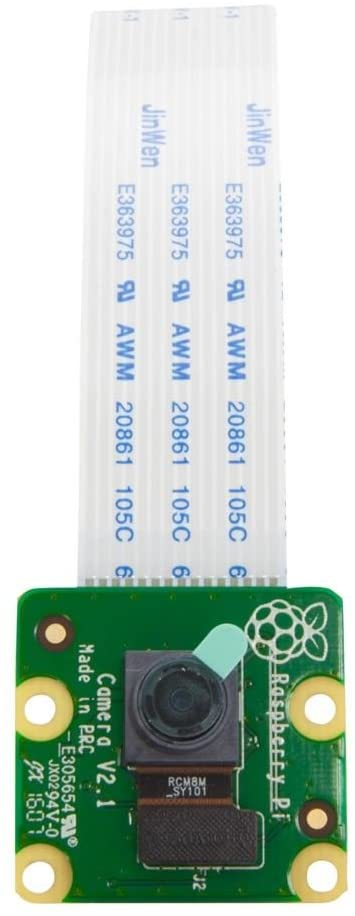
\includegraphics[scale=0.1]{module_cam.jpg}
            \caption{Module de capture vidéo (Raspberry Pi) V2}
        \end{figure}
        
    \section{Montage, Installation et Configuration}
        % du unpack au systeme fonctionnel ... Méthodo, doc , etc ...
        Il faut savoir que le Raspberry Pi et son module caméra arrive séparément ce qui signifie que le module est pas monté sur le Raspberry Pi.
        Le Raspberry Pi arrive sans son système pré-installé.
            \subsection{Montage du matériel}
            Le Raspberry Pi possède un port CSI 'Camera Serial Interface' (signifiant en anglais interface série pour caméra, CSI) est un standard d'interface électronique entre une caméra (un capteur ou une source vidéo) et un microprocesseur.

            \begin{figure}[h]
                \centering
                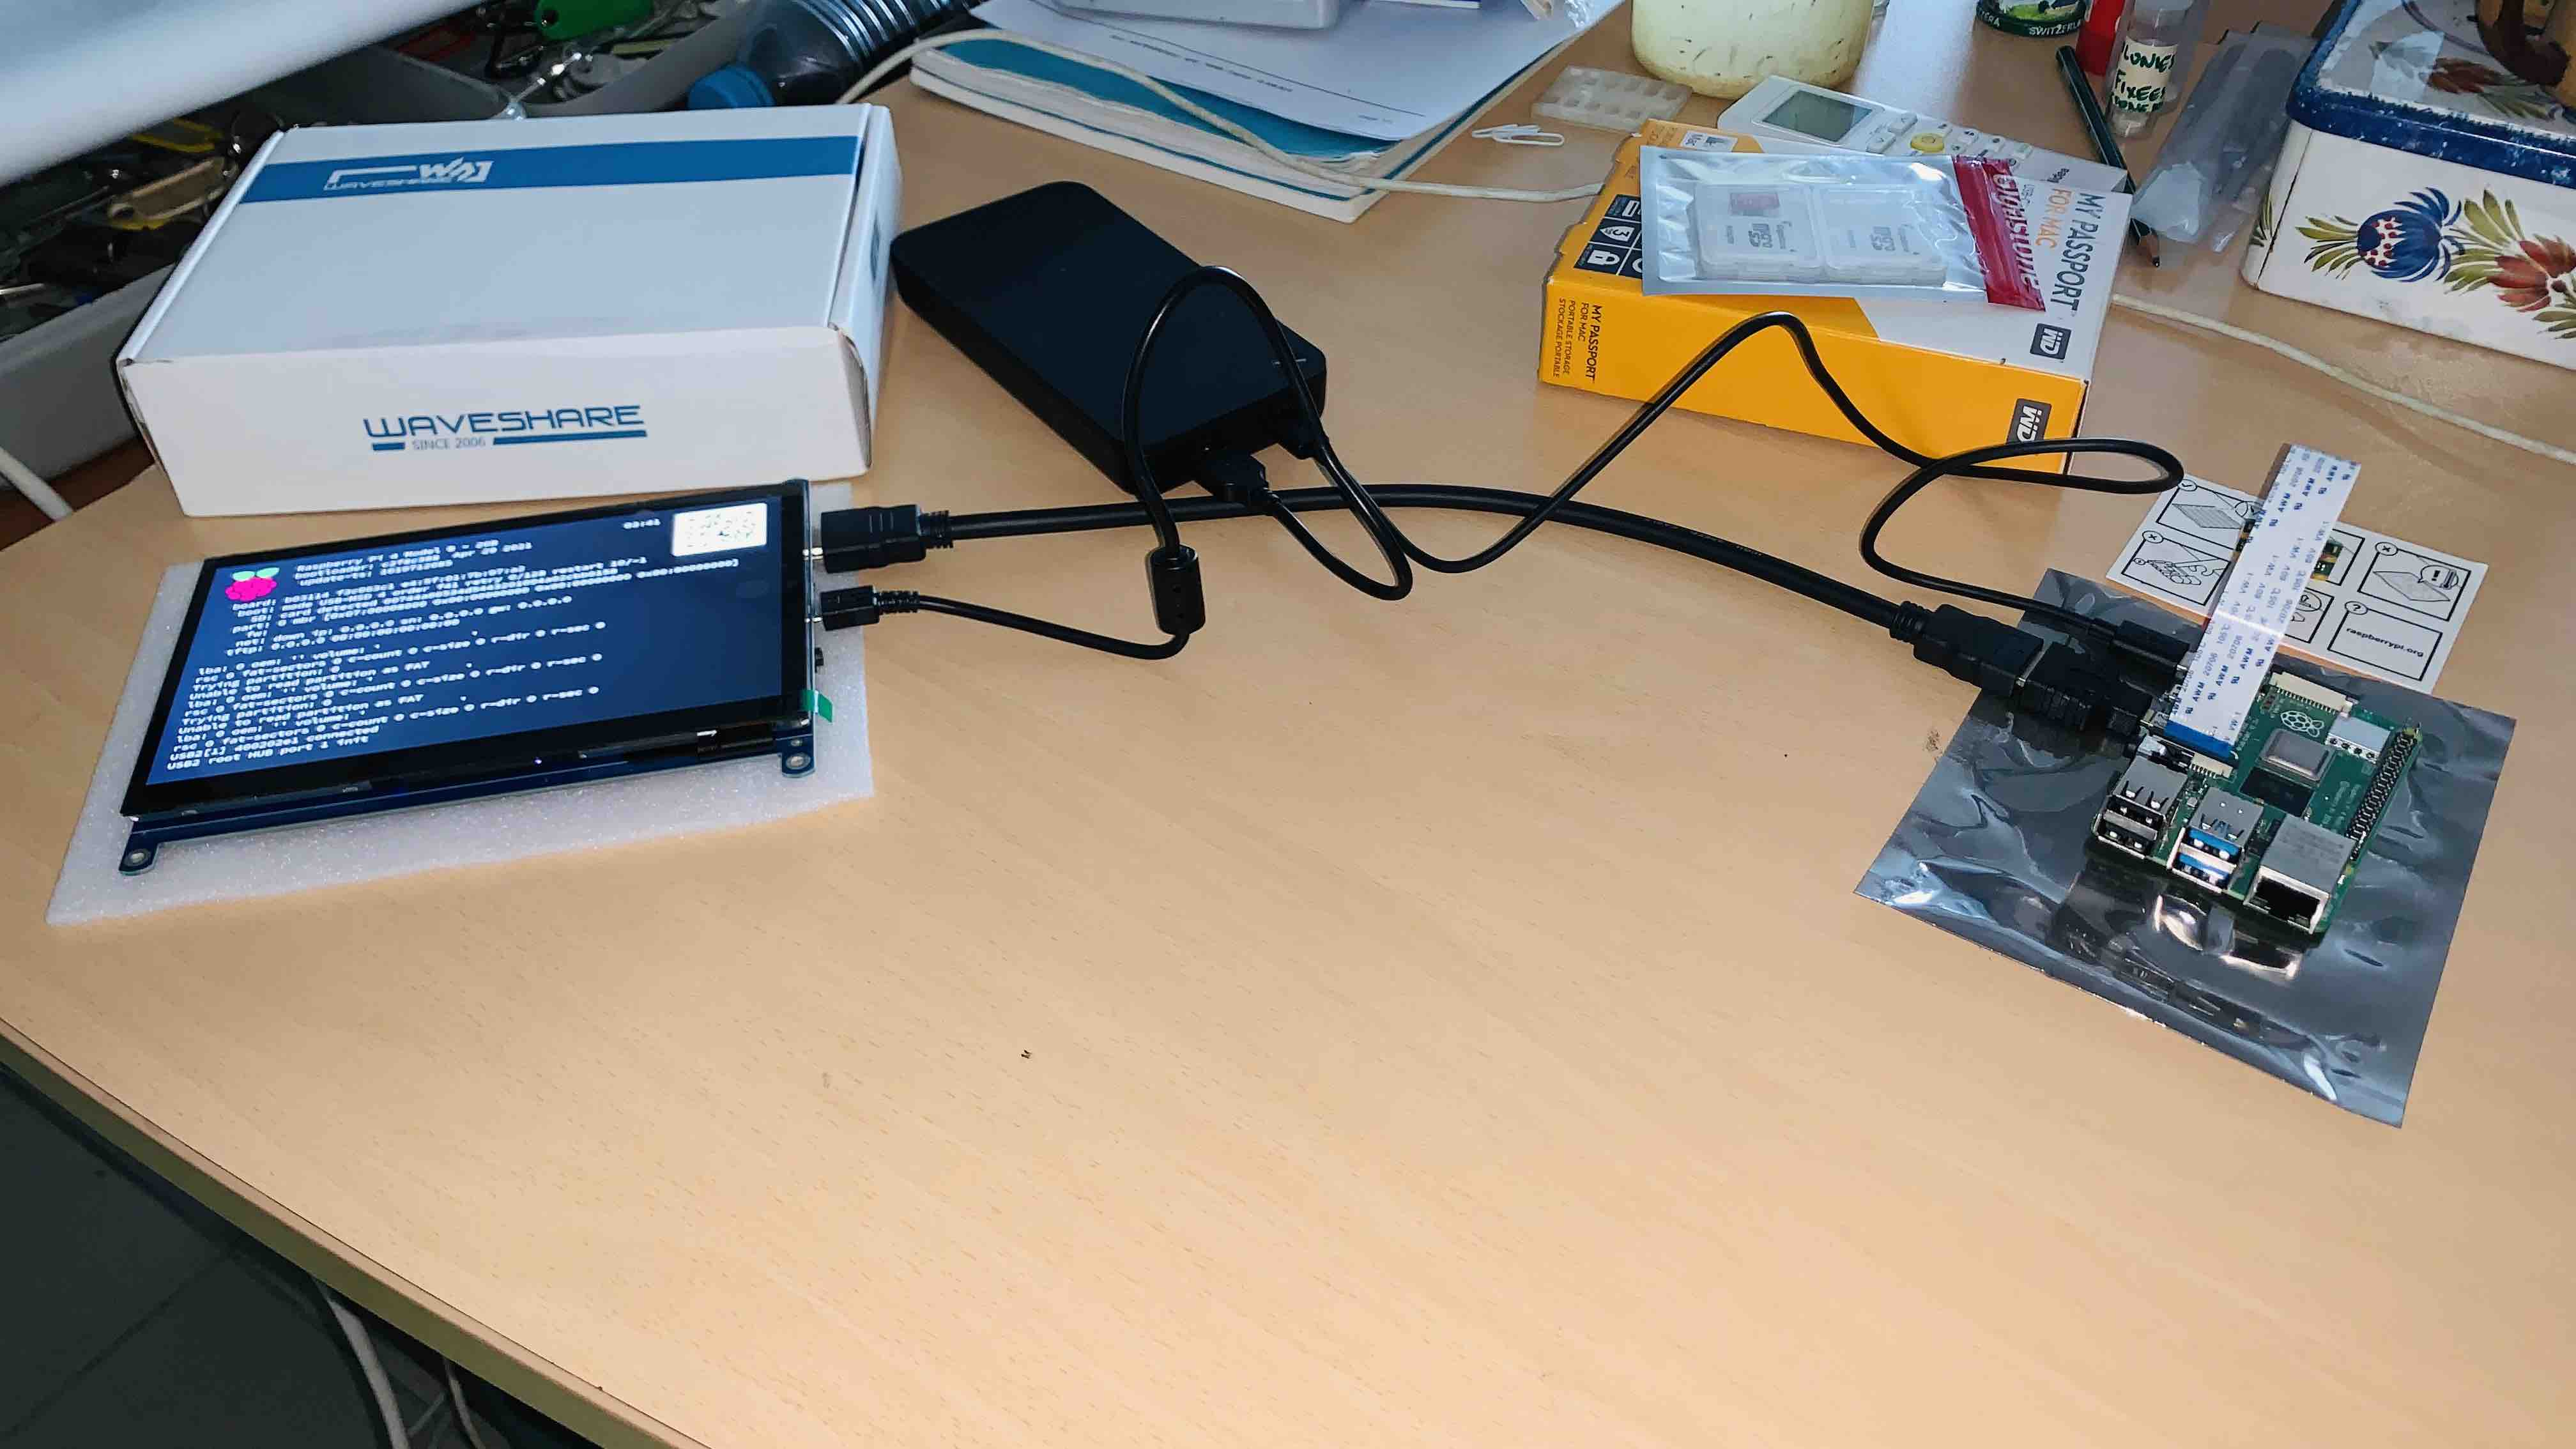
\includegraphics[scale=0.04]{unpack.jpeg} 
                \caption{Matériel assemblé et prêt à l'emploi}
            \end{figure}

            \vspace{0.2cm}

            Afin de pouvoir utiliser le module camèra il nous faut donc inseré la nappe de connecteur de la caméra dans le port CSI du Raspberry Pi.
            \subsection{Installation du matériel}
            % Qu'est ce que linux
            Le système étant pas pré-installé, il nous faut installer le système d'exploitation.
            Pour ce faire nous allons utiliser Raspberry Pi Imager.

            \vspace{0.2cm}

            \begin{flushleft}
                Raspberry Pi Imager est le moyen rapide et facile d'installer Raspberry Pi OS sur une microSD.\\[0.2cm]

                Il nous faut télécharger le fichier d'installation sur le site web Raspberry.com et de l'installer.\\[0.2cm]

                Nous obtenons alors l'aperçu de la figure 4.4.\\[0.2cm]
                Comme nous pouvons le voir sur cette figure, le logiciel nous demande de choisir l'OS que nous souhaitons installer.
                On lui indique donc que nous voulons installer l'OS Raspbian en 32 bits. Et on choisit notre stockage qui dans notre cas est une microSD.

                \vspace{0.2cm}

                Une fois cela fait, on lance l'écriture, le logiciel va télécharger l'OS et installer l'OS sur la microSD.


            \begin{figure}[t]
                \centering
                \includegraphics[scale=0.3]{Installation_1.png} 
                \caption{Interface "Raspberry Pi Imager"}
            \end{figure}


            \end{flushleft}
    
            \subsection{Configuration du matériel}
            Avant de pouvoir utiliser le module caméra, activer l'interface caméra.
            Pour ce faire nous allons utiliser la commande \textbf{sudo raspi-config}.

            \begin{figure}[h]
                \centering
                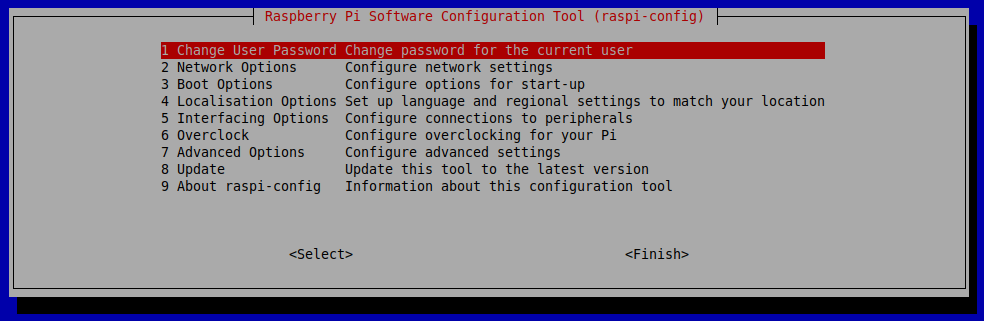
\includegraphics[scale=0.3]{raspi-config.png} 
                \caption{Interface "raspi-config"}
            \end{figure}

            \begin{flushleft}
                
                Une fois dans \textbf{Raspi-config}, nous allons choisir la section \textbf{Interface section}.
            
                \begin{figure}[h]
                    \centering
                    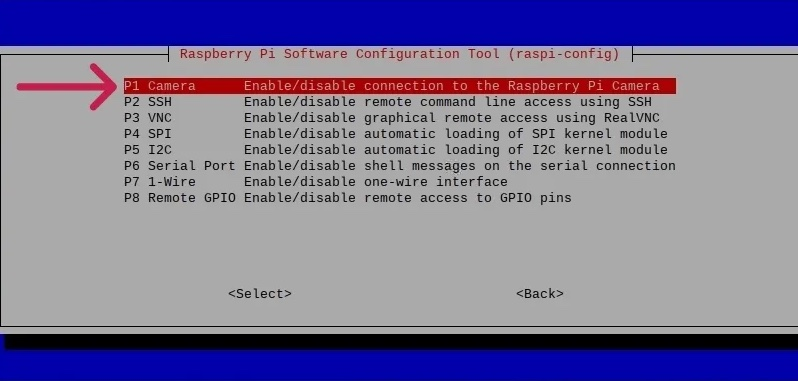
\includegraphics[scale=0.3]{raspiconfig-camera-option.jpg} 
                    \caption{camera option (raspi-config)}
                \end{figure}

                On selectionne \textbf{P1 Camera} et on met sur \textbf{Enable}.

                \vspace{0.2cm}

                Une fois cela fait on peut quitter \textbf{Raspi-config} et tester si la caméra est bien activée et fonctionne correctement.

                \vspace{0.2cm}

                Pour ce faire, on ouvre le terminal et on tape la commance suivante :

                \begin{flushleft}
                    \begin{lstlisting}[language=bash]
                        raspistill -o Desktop/image.jpg
                    \end{lstlisting}
                \end{flushleft}

                Cette commande nous permet de prendre une photo et de la sauvegarder dans le dossier Desktop.

                \vspace{0.2cm}

                La photo est bien prise. De ce fait la caméra est opérationnelle.

                Nous pouvons tout de même essayer de faire une vidéo.

                \begin{flushleft}
                    \begin{lstlisting}[language=bash]
                        raspivid -o Desktop/video.h264
                    \end{lstlisting}
                \end{flushleft}

                Cette commande nous permet de prendre une vidéo et de la sauvegarder dans le dossier Desktop.

                \vspace{0.2cm}

                La vidéo est bien prise. Donc tout est fonctionnel.
                
            \end{flushleft}

    \section{Choix des technologies}
        Pour le choix du langage de programmation, je me suis basé sur les langages de programmation les plus classés pour le (Raspberry Pi) système d'exploitation Raspbian.
        Lors de ma recherche 5 langages de programmation en sont sortis : 

        \vspace{0.2cm}

        \begin{itemize}
            \item Python
            \item C
            \item Java/BlueJ
            \item Perl
            \item Scratch
        \end{itemize}

        \begin{flushleft}
            On peut voir que le langage Python est le plus utilisé pour le (Raspberry Pi) système d'exploitation Raspbian.

            Ce qui est normal, car le Pi dans "Raspberry Pi" signifie "Python". Il a donc le mérite d'être le choix par défaut.

            Afin de pouvoir me décider sur le langage de programmation, il me faut chercher la compatibilité des API pour la camera. 

            Il s'avère que l'API PiCamera est installer par défaut sur le système d'exploitation Raspbian.

            Puisque le langage Python et l'API PiCamera sont compatibles, et installer par défaut sur le système d'exploitation Raspbian, il est possible de choisir le langage Python.
        
            Même si le langage de programmation JavaScript ne figure pas dans cette liste, il est très utilisé, il est donc très intéressant de le choisir.
            Avec electron et nodejs, nous pouvons très bien créer une application multiplatforme.\\[0.2cm]
            De plus, l'API PiCamera est disponible pour le langage JavaScript.
        
            Mais par manque de temps, nodejs et electron ne sont pas installés par défaut sur le Raspberry Pi.\\[0.2cm]
        
            De ce fait nous allons utiliser le langage Python pour la programmation du logiciel.
            
            Python est un langage de programmation interprété, multi-paradigme et multiplateformes. Il favorise la programmation impérative structurée, fonctionnelle et orientée objet.
            
            % définir le multi-paradigme
            % définir le multiplateformes
            % Programattion interprété, structurée, fonctionnelle et orientée objet
        \end{flushleft}

    % Qu'est ce que le langage Python ?
    
    \section{Réalisation de l'application}
        Avant toutes choses, nous allons importer les modules nécessaires.
        Nous allons utiliser les modules :
        \begin{itemize}
            \item \textbf{picamera}
            \item \textbf{tkinter}
            \item \textbf{datetime}
            \item \textbf{os}
            \item \textbf{time}
        \end{itemize}

        \begin{flushleft}
            Maintenant que nos modules sont importés, nous allons créer une maquette du menu principal de l'application.
            Cette maquette nous permettra d'avoir un aperçu de l'application.
            Et nous permettra de concevoir le GUI de l'application à l'aide de Tkinter.            
        \end{flushleft}

        \subsection{Création de l'interface graphique}
            \begin{figure}[h]
                \centering
                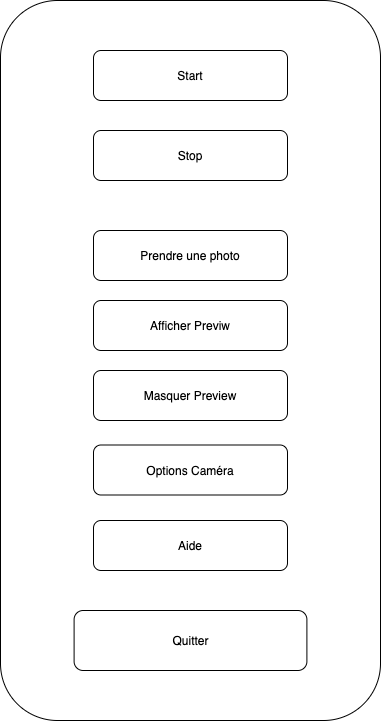
\includegraphics[scale=0.3]{maquette.png} 
                \caption{Maquette de l'application}
            \end{figure}

            \begin{flushleft}
                Nous allons créer 5 classes pour notre GUI qui sont :
                \begin{itemize}
                    \item \textbf{class} \textit{App}
                    \item \textbf{class} \textit{AppPhotoSection}
                    \item \textbf{class} \textit{AppOptionsSection}
                    \item \textbf{class} \textit{AppUtilitySection}
                    \item \textbf{class} \textit{AppHelpSection}
                \end{itemize}
                
                La classe \textit{App} est la classe principale de notre application.
                C'est ici que nous allons définir la taille de la fenêtre, la couleur de fond, le titre de la fenêtre, le logo de l'application, ... .
                C'est également dans cette classe que nous allons lancer notre menu principal par la méthode : \textbf{def \_\_init\_\_(self, master)}.
            
                La méthode \_\_init\_\_ peut être appelée lorsqu'un objet est créé à partir de la classe, et un accès est nécessaire pour initialiser les attributs de la classe.

                \vspace{0.2cm}

                Le menu principal est représenté par la maquette de la figure 4.8.

                \vspace{0.2cm}

                Les 4 autres class sont les classes qui représentent les sections de l'application.
                Lorsque que l'utilisateur clique sur un des boutons du menu principal, il se rend dans la section correspondante.

                % tk.frame 

            \end{flushleft}
        
        \vspace{1cm}

        \subsection{Fonction Start Recording}
            Afin de réaliser l'application, nous allons commencer par concevoir la fonction coeur de l'application.
            C'est à dire la fonction qui va nous permettre de lancer un enregistrement et de l'arrêter.    
            Cette fonction, son fonctionnement est érigés par la figure 4.9
            \begin{figure}[h]
                \centering
                \includegraphics[scale=0.4]{diagram_activité_enregistrement.png} 
                \caption{Diagramme d'activité de la fonction "Démarer un Enregistrement"}
            \end{figure}

            \begin{flushleft}
                D'après notre diagramme d'activité, il nous faut commencer l'enregistrement lorsque l'utilisateur clique sur le bouton "Start".

                \vspace{0.2cm}

                Avant de pouvoir démarrer un enregistrement, il faut initialiser la caméra, pour cela, la documentation nous indique une fonction pour cela qui est : \textbf{camera = PiCamera()}.

                Une fois la caméra initialisée, nous pouvons commencer à traiter la demande de l'utilisateur.

                
                \textbf{AskForSaveFile} est une fonction de tkinter qui va nous permettre de demander à l'utilisateur de saisir un nom de fichier et de lui permettre de choisir l'emplacement de sauvegarde.

                \vspace{0.2cm}

                Une fois que l'utilisateur a saisi le nom de fichier, nous pouvons commencer à enregistrer avec la fonction de l'API PiCamera : \textbf{camera.start\_recording(nomDuFichier, format)}.
                L'enregistrement restera actif tant que l'utilisateur ne clique pas sur le bouton "Stop".
                L'arrêt de l'enregistrement se fait avec la fonction de l'API PiCamera : \textbf{camera.stop\_recording()}.

                \vspace{0.2cm}
                Lors des tests, nous avons remarqué qu'arrêter l'enregistrement de manière manuelle est parfois pas très optimale.
                Nous avons donc décider de créer une fonction nous permettant de stopper de manière automati l'enregistrement.

                \vspace{0.2cm}

                Il s'agit de permettre à l'utilisateur de saisir un temps en minutes et de lancer l'enregistrement.

                \vspace{0.2cm}

                Le temps saisie en minute de l'utilisateur sera converti en secondes.

                De ce fait, l'API PiCamera nous permet de définir le temps d'enregistrement en secondes avec la fonction : \textbf{camera.wait\_recording(tempsEnSeconde)}.
                
                \vspace{0.2cm}

                Cependant cette fonction possède un défaut, elle agit comme une fonction \textbf{wait()} classique. De ce fait, durant l'enregistrement, l'utilisateur ne peut pas interagir avec l'application.

                Une fois que nous n'utilison plus la caméra, nous pouvons couper toute utilisation de la caméra avec la fonction de l'API PiCamera : \textbf{camera.close()}.

            \end{flushleft}


        \subsection{Prendre une capture}
        La fonction prendre une capture est une fonction qui va nous permettre de prendre une photo.
        Cette fonction est érigée par la figure 4.10.
        \begin{figure}[ht]
            \centering
            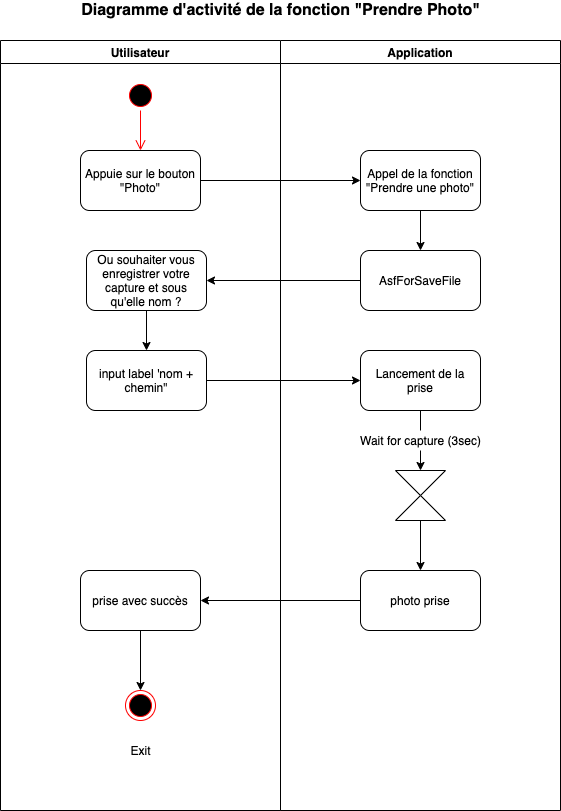
\includegraphics[scale=0.4]{diagram_3.png} 
            \caption{Diagramme d'activité de la fonction "Prendre une capture"}
        \end{figure}


        \begin{flushleft}
            Contrairement à la fonction \textbf{Démarrer un Enregistrement}, cette fonction est plus simple dans l'ensemble de son fonctionnement.

            \vspace{0.2cm}

            Tout d'abord, comme nous l'avons vu pour la fonction \textbf{Démarrer un Enregistrement}, nous allons initialiser la caméra.

            \vspace{0.2cm}
    
            Une fois celle-ci initialisée, nous allons demander à l'utilisateur de saisir un nom de fichier et l'emplacement de sauvegarde.

            \vspace{0.2cm}
    
            Une fois cela fait, il nous faudra pré-chauffer la caméra afin de pouvoir lancer la capture d'image.
            
            \vspace{0.2cm}
    
            Avec la fonction \textbf{sleep()}, nous allons attendre un certain délai avant de lancer la capture.
            Pour le pré-chauffahe, 2-3 secondes suffiront.

            \vspace{0.2cm}
    
            Une fois cela fait, nous pouvons lancer la capture avec la fonction de l'API \textbf{camera.capture(nomDuFichier, format)}.
            
            \vspace{0.2cm}

            Nous avons également décidé d'ajouter une fonction permettant de prendre des photos en continu.

            \vspace{0.2cm}

            Nous allons donc créer une fonction permettant de prendre des photos en continu.
            Afin de pouvoir faire cela, nous allons demander à l'utilisateur de saisir un nom de fichier et l'emplacement de sauvegarde comme précédemment.
            Mais avant cela, nous demandons à l'utilisateur de choisir le nombre de photos à prendre.

            \vspace{0.2cm}

            Pour cela, nous utilison une boucle telle que : 
            \begin{verbatim}
                for nomDuFichier in camera.record_sequence(
                    '%d.h264' % i for i in range(1, nombreDePhoto)):
                camera.wait_recording(6)
            \end{verbatim}

            Tant que le nombre de photos voulue n'est pas atteint, nous allons continuer à prendre des photos toutes les 6 secondes.

            \vspace{0.2cm}

            Nous avons mis un délai de 6 secondes entre chaque photo afin que la prise ne soit pas exactement identique à la précédente.
        \end{flushleft}

        

        \subsection{Travail en laboratoire}
        Tout le système que nous avons crée jusqu'à maintenant est destiné à être utilisé dans un laboratoire.

        \begin{figure}[ht]
            \centering
            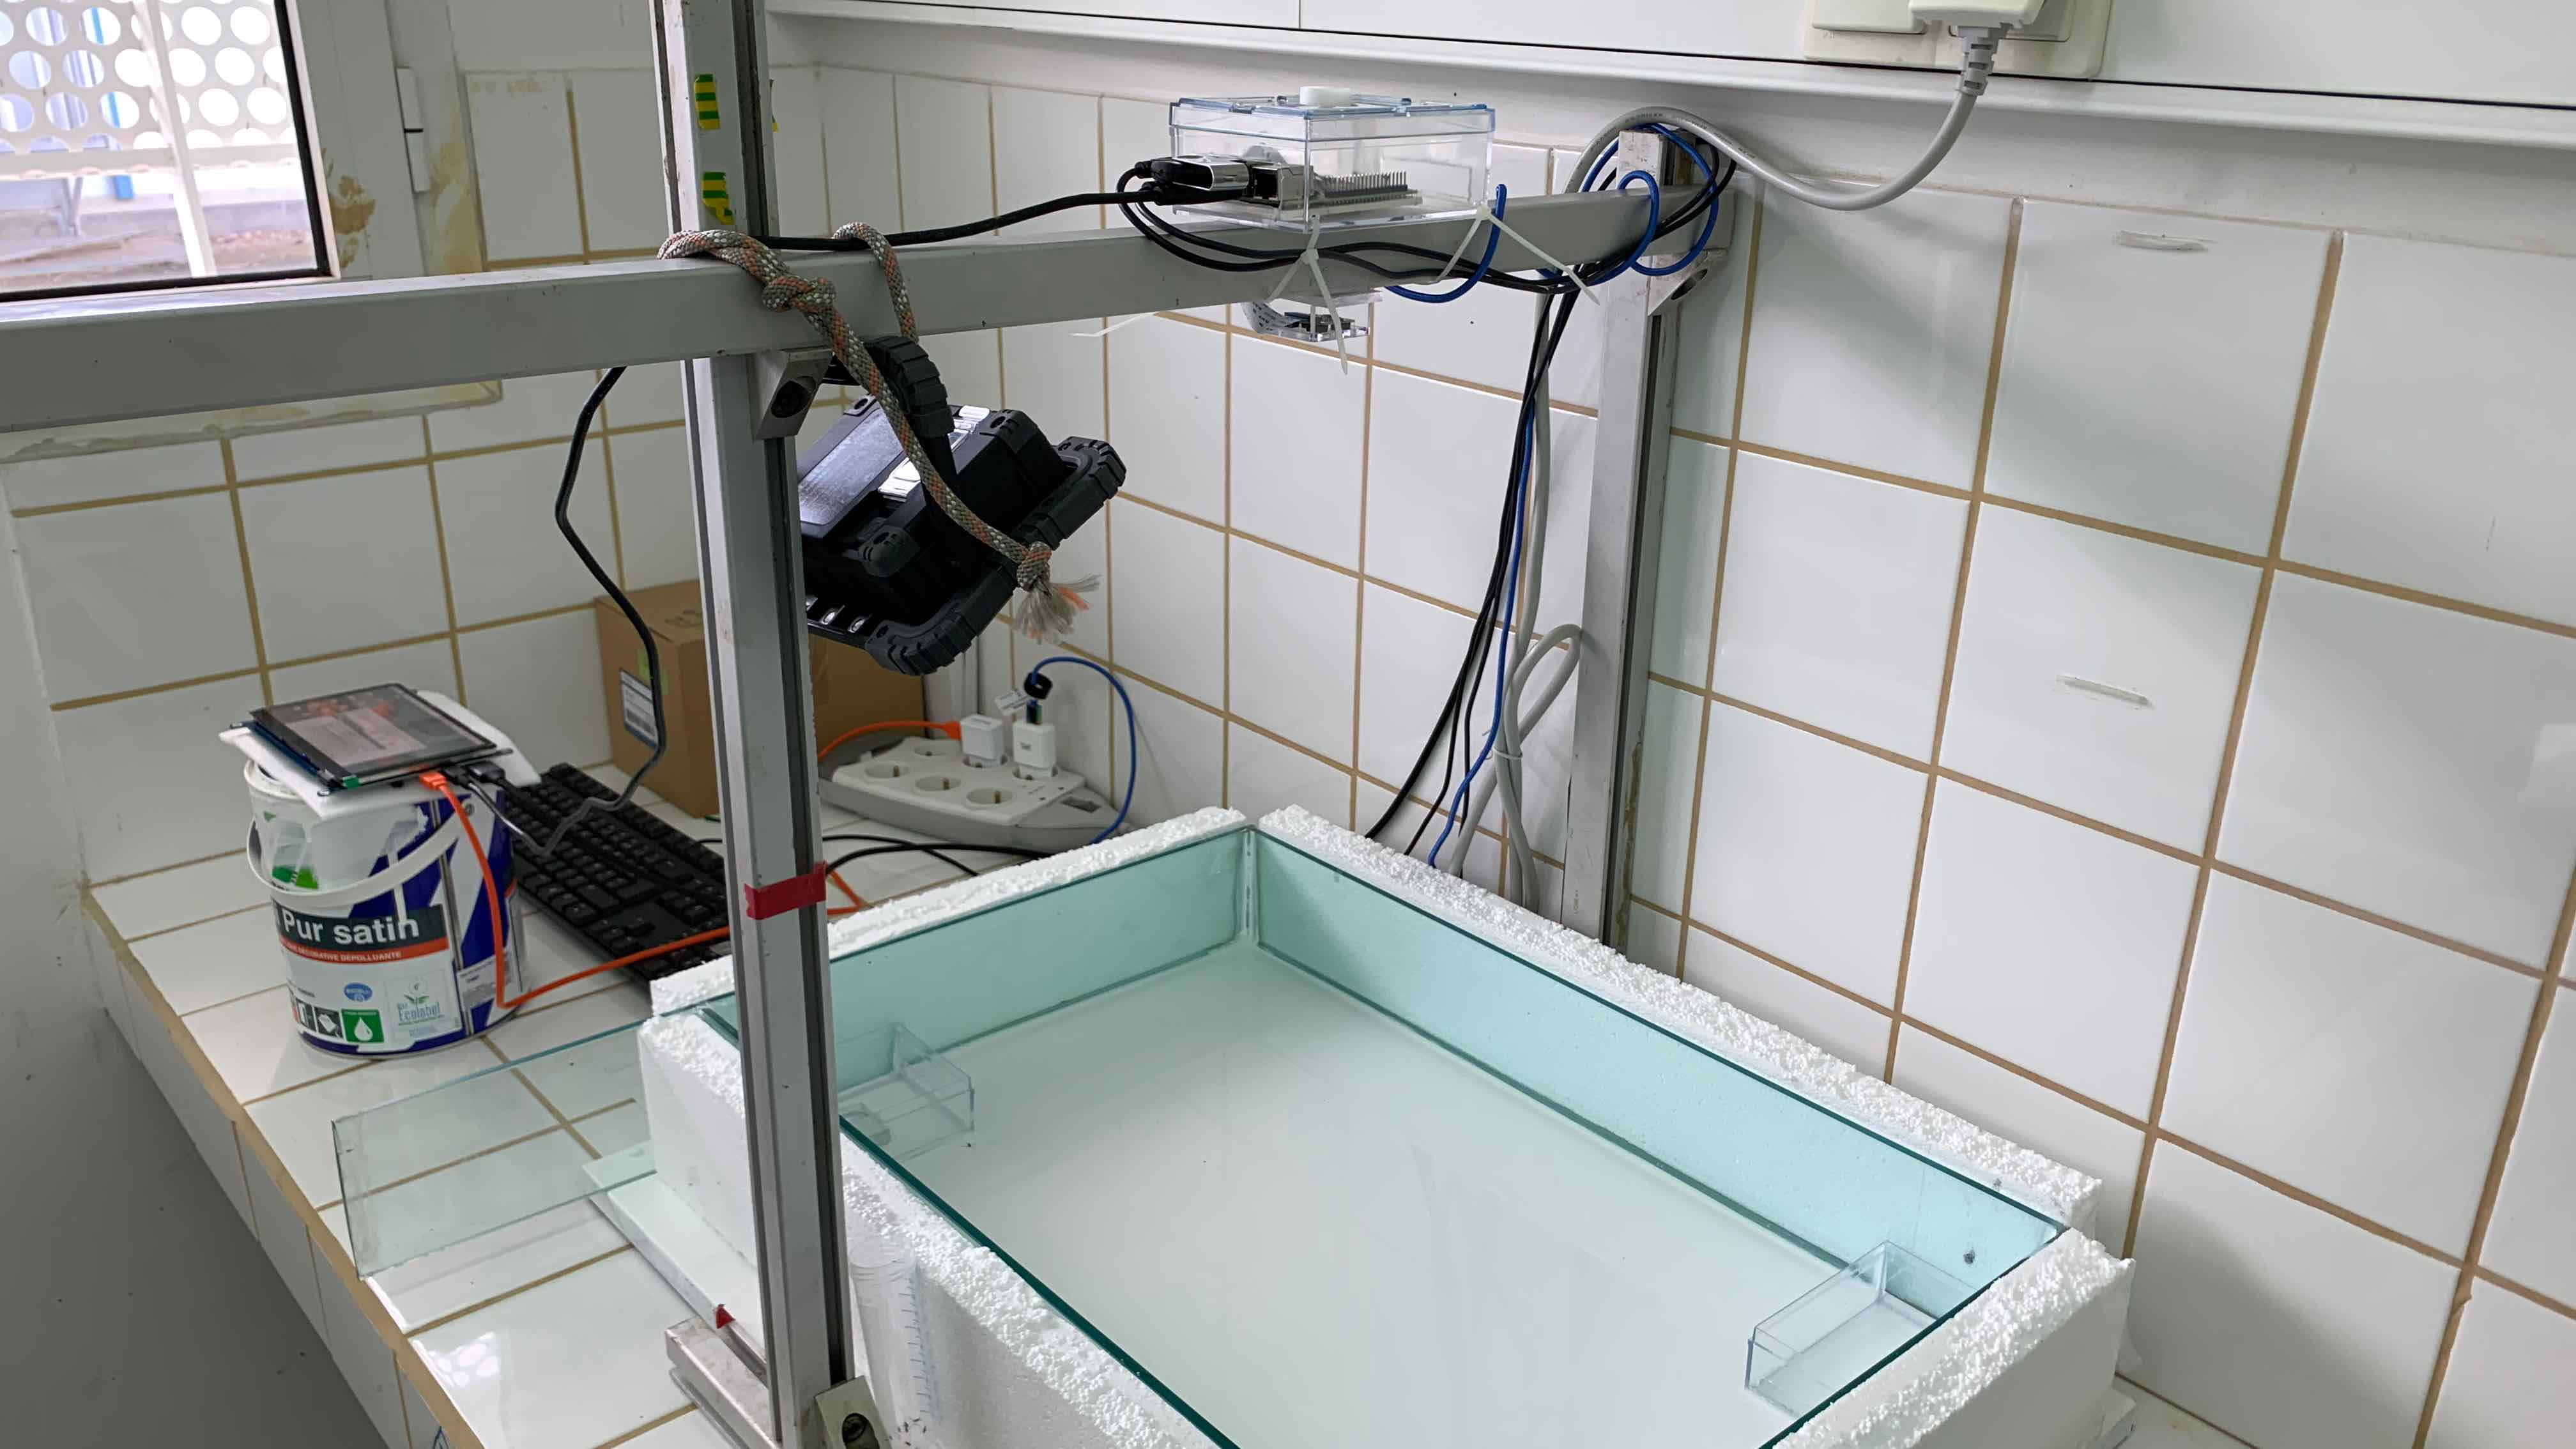
\includegraphics[scale=0.09]{setup.jpeg} 
            \caption{Le dispositif installé dans le laboratoire}
        \end{figure}

        J'ai eu l'occasion de partir à la recherche de Gérridés dans la Mangrove de la Guadeloupe et d'en attraper a l'épuisette (voir Figure 3.2).
        \begin{figure}[ht]
            \centering
            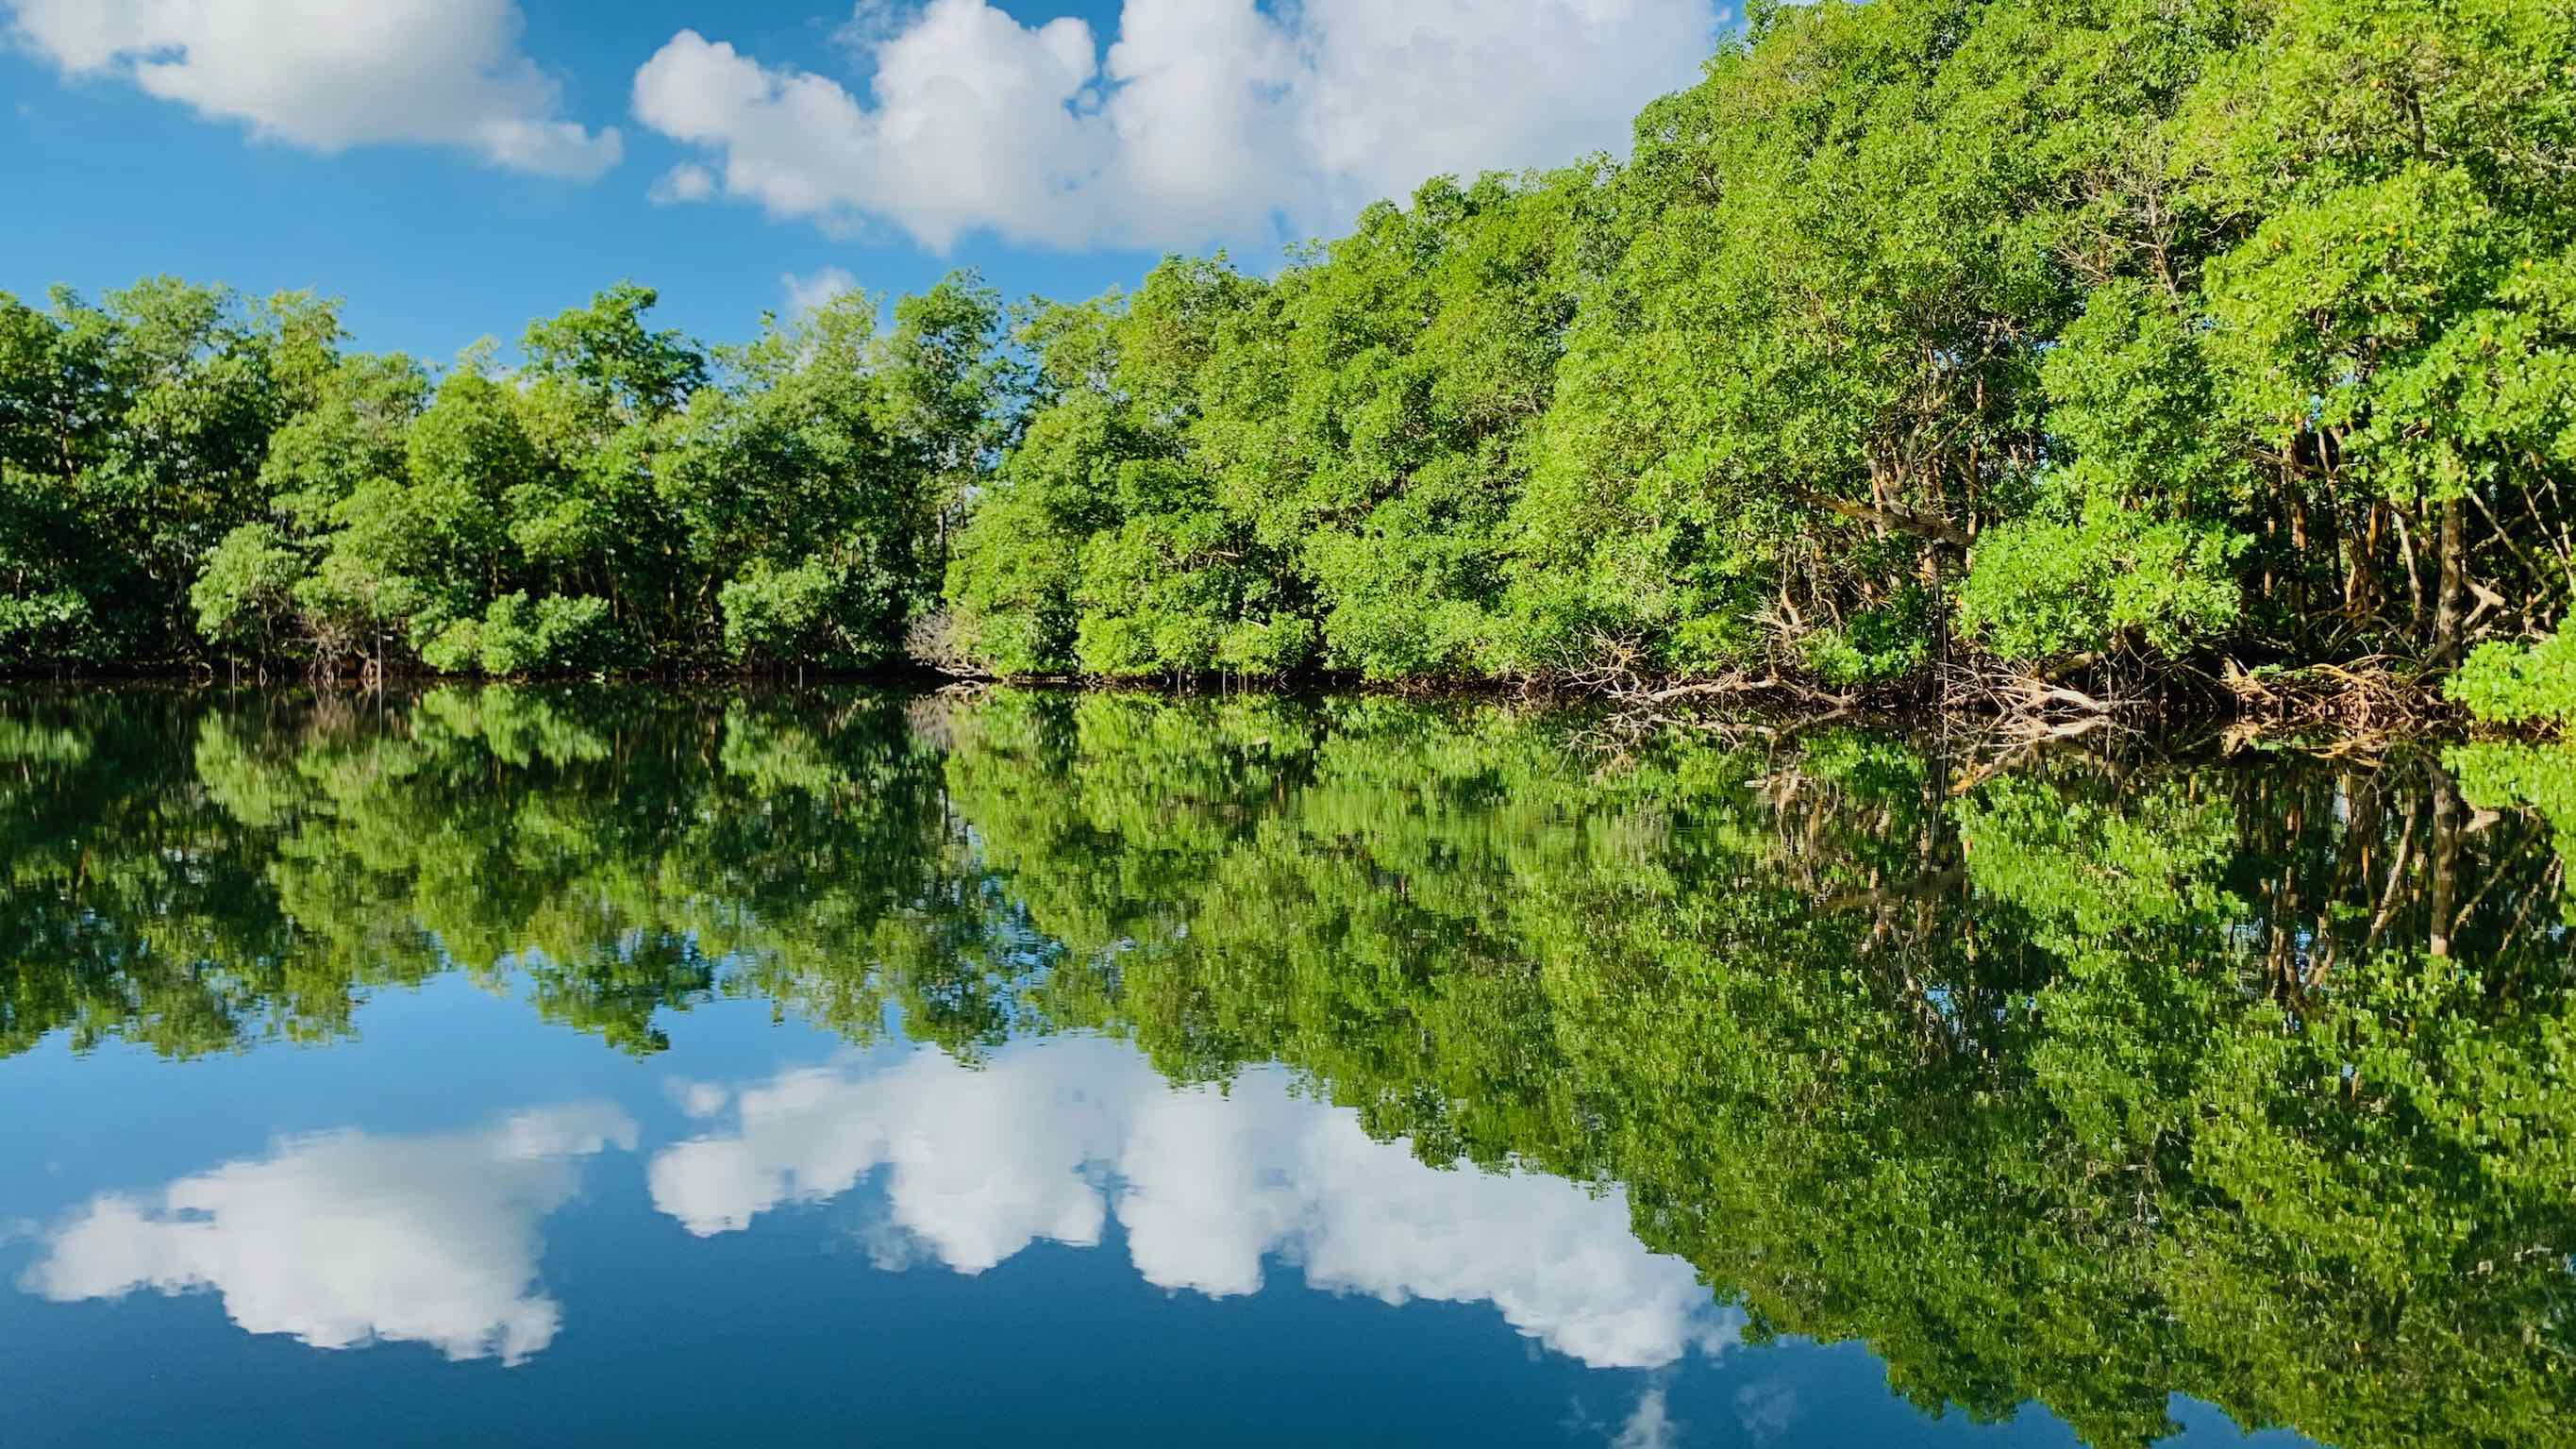
\includegraphics[scale=0.04]{mangrove.jpeg}
            \caption{Mangrove de la Guadeloupe}
        \end{figure}
        
        